\section{Results and Discussion}

Using what we have established in previous sections provides the necessary tools to simulate the double pendulum's complex dynamics. With the equations of motion derived via the Lagrangian and the Runge-Kutta solver implemented in Julia, we now turn to the simulation results.

\subsection{Numerical Results}
To verify the chaotic nature of the double pendulum, we simulated the system's time evolution using the RK4 integrator derived in Section 3. We specifically investigated the system's sensitivity to initial conditions.

We initialized two \textit{almost} identical double pendulum systems (sharing identical lengths $l_1,l_2$ and masses $m_1,m_2$) with initial angles differing by a microscopic perturbation, $\epsilon$:
\[\Theta_A=(\theta_1,\theta_2)\quad\text{and}\quad \Theta_B=(\theta_1+\epsilon,\theta_2)\]
where $\epsilon = 10^{-5}$ degrees.

\figref{10-5} illustrates the trajectories of these two systems over time. During the initial phase of the simulation, the deviation caused by the perturbation appears negligible, and the systems move in unison. However, as the system evolves, the non-linear coupling terms in the equations of motion, specifically those derived in \eqref{eq:rearr1}, cause this infinitesimal difference $\epsilon$ to propagate and grow exponentially for some time.

\begin{figure}[h]
  \centering
    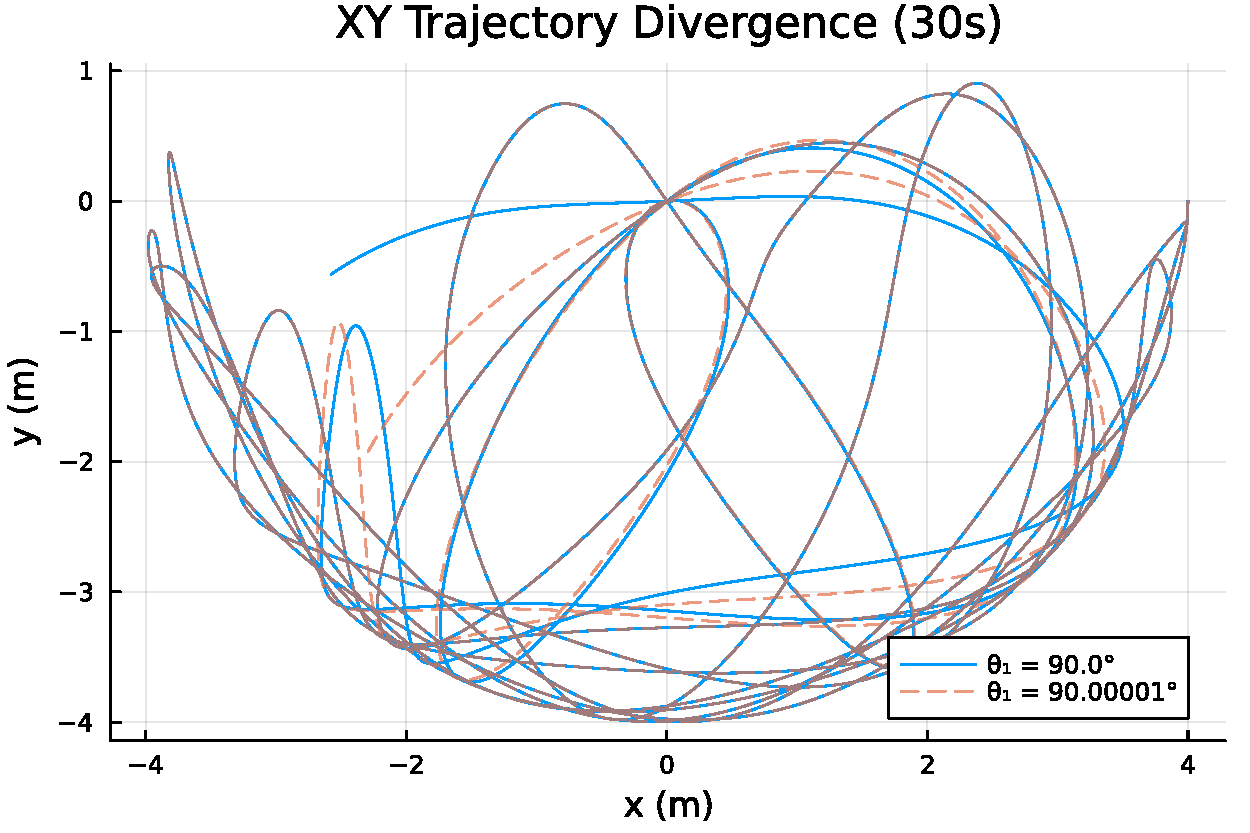
\includegraphics[width=0.8\textwidth]{Figures/xy_divergence.pdf}
    \caption{Divergence of trajectories with initial conditions differing by $10^{-5}$ degrees.}
    \figlabel{10-5}
\end{figure}

By the end of the simulation, the two pendulums exhibit completely uncorrelated states, occupying different regions of the configuration space despite being governed by the same deterministic laws. This confirms that while the double pendulum is deterministic (fully described by Equations \ref{ddtheta1} and \ref{ddtheta2}), it is practically unpredictable over long time horizons due to this extreme sensitivity.

Plotting the angular difference $\Delta\theta$ between the two systems further illustrates this chaotic dissociation. As shown in \figref{dt}, the error does not grow linearly but exhibits rapid, unpredictable fluctuations, the peaks of which grow exponentially, characteristic of the butterfly effect.

\begin{figure}[h]
  \centering
    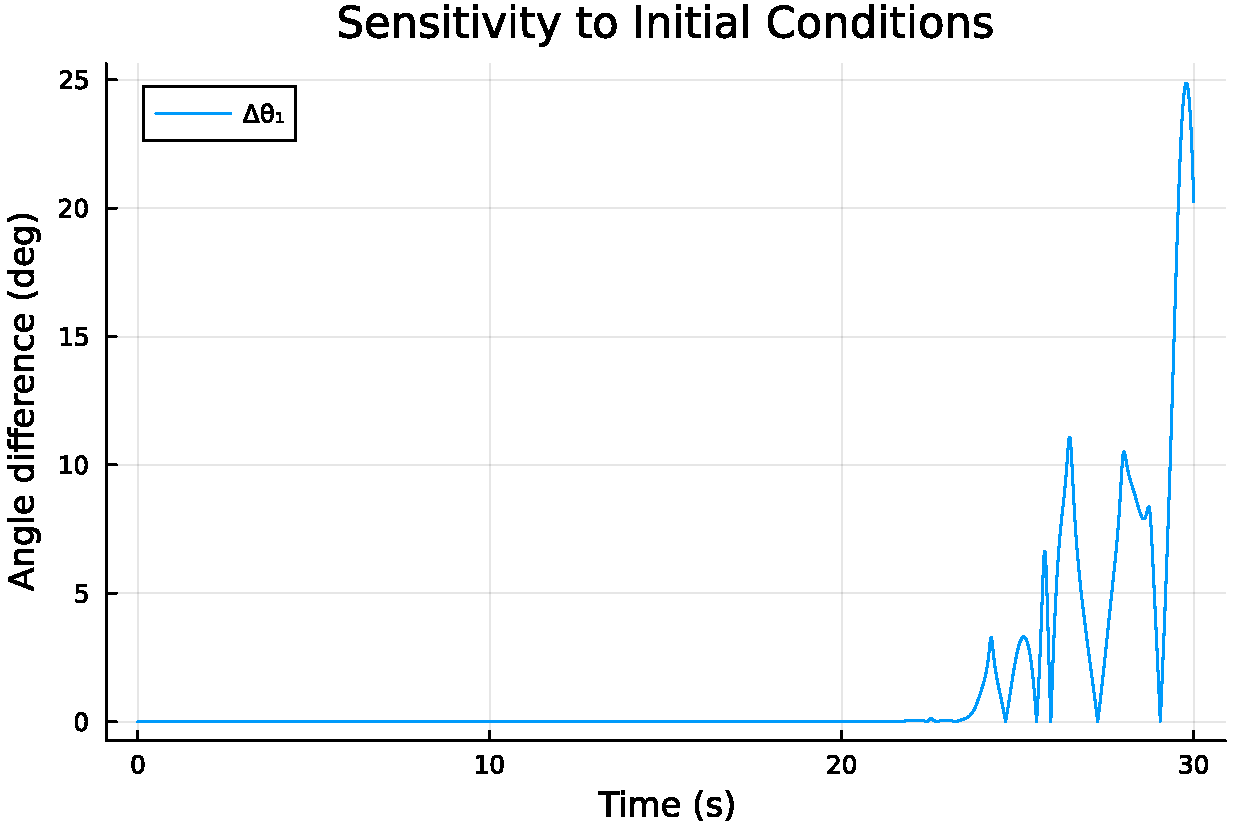
\includegraphics[width=0.8\textwidth]{Figures/dt.pdf} 
    \caption{Evolution of the angular difference $\Delta\theta$ between the two systems over time.}
    \figlabel{dt}
\end{figure}

\subsection{Conclusion}
In this project, we modeled the dynamics of a double pendulum, moving from the theoretical physical setup to a full numerical simulation. By utilizing the Lagrangian formulation, we avoided the vector complexity of Newtonian mechanics and directly derived the coupled non-linear equations of motion.

We transformed these second-order differential equations into a state-space representation suitable for computational solving. The implementation of the fourth-order Runge-Kutta (RK4) method allowed us to accurately approximate the solution, maintaining numerical stability even as the system entered chaotic regimes.

The results validate that simple physical systems can exhibit complex, non-linear behavior. The visualization of the trajectory divergence serves as a concrete demonstration of deterministic chaos, satisfying the primary objective of this study. Future work could involve solving triple or \(n\)-pivot pendulums. This would require much higher dimension vector fields to incorporate into the Runge-Kutta methods. 
